\chapter{Aplikacja demonstracyjna}

W tym rozdziale zaprezentuję jak stworzyć prostą aplikację na iOS wykorzystującą wcześniej przedstawioną bibliotekę \textbf{EPUBKit}. Pierwszym krokiem będzie otwarcie Xcode i stworzenie nowego projektu, analogicznie do tego co opisano w rozdziale czwartym. W tym przypadku jednak wybierzemy szablon \textit{Single View Application} i damy nazwę projektowi \textbf{EPUBDemo}\cite{UsingSwiftWithCocoaAndObjectiveC}. Po wybraniu lokalizacji w której chcemy zapisać aplikację, ukazuje nam się widok projektu w Xcode IDE tak jak miało to miejsce w przypadku tworzenia biblioteki. Biorąc pod uwagę demonstracyjne przeznaczenie aplikacji zamierzam ograniczyć się do minimum i skupić się na samej integracji z biblioteką oraz wykorzystanie \textit{API} które jest przez nią dostarczane. Chcę przedstawić proces tworzenia widoków z których składa się aplikacja na iOS, rozpoczynając od omówienia wykorzystywanego wzorcu architektonicznego \textit{MVC}, przejdę do opisania elementów interfejsu użytych w aplikacji oraz klas które je reprezentują.

\begin{figure}[ht!]
  \centering
  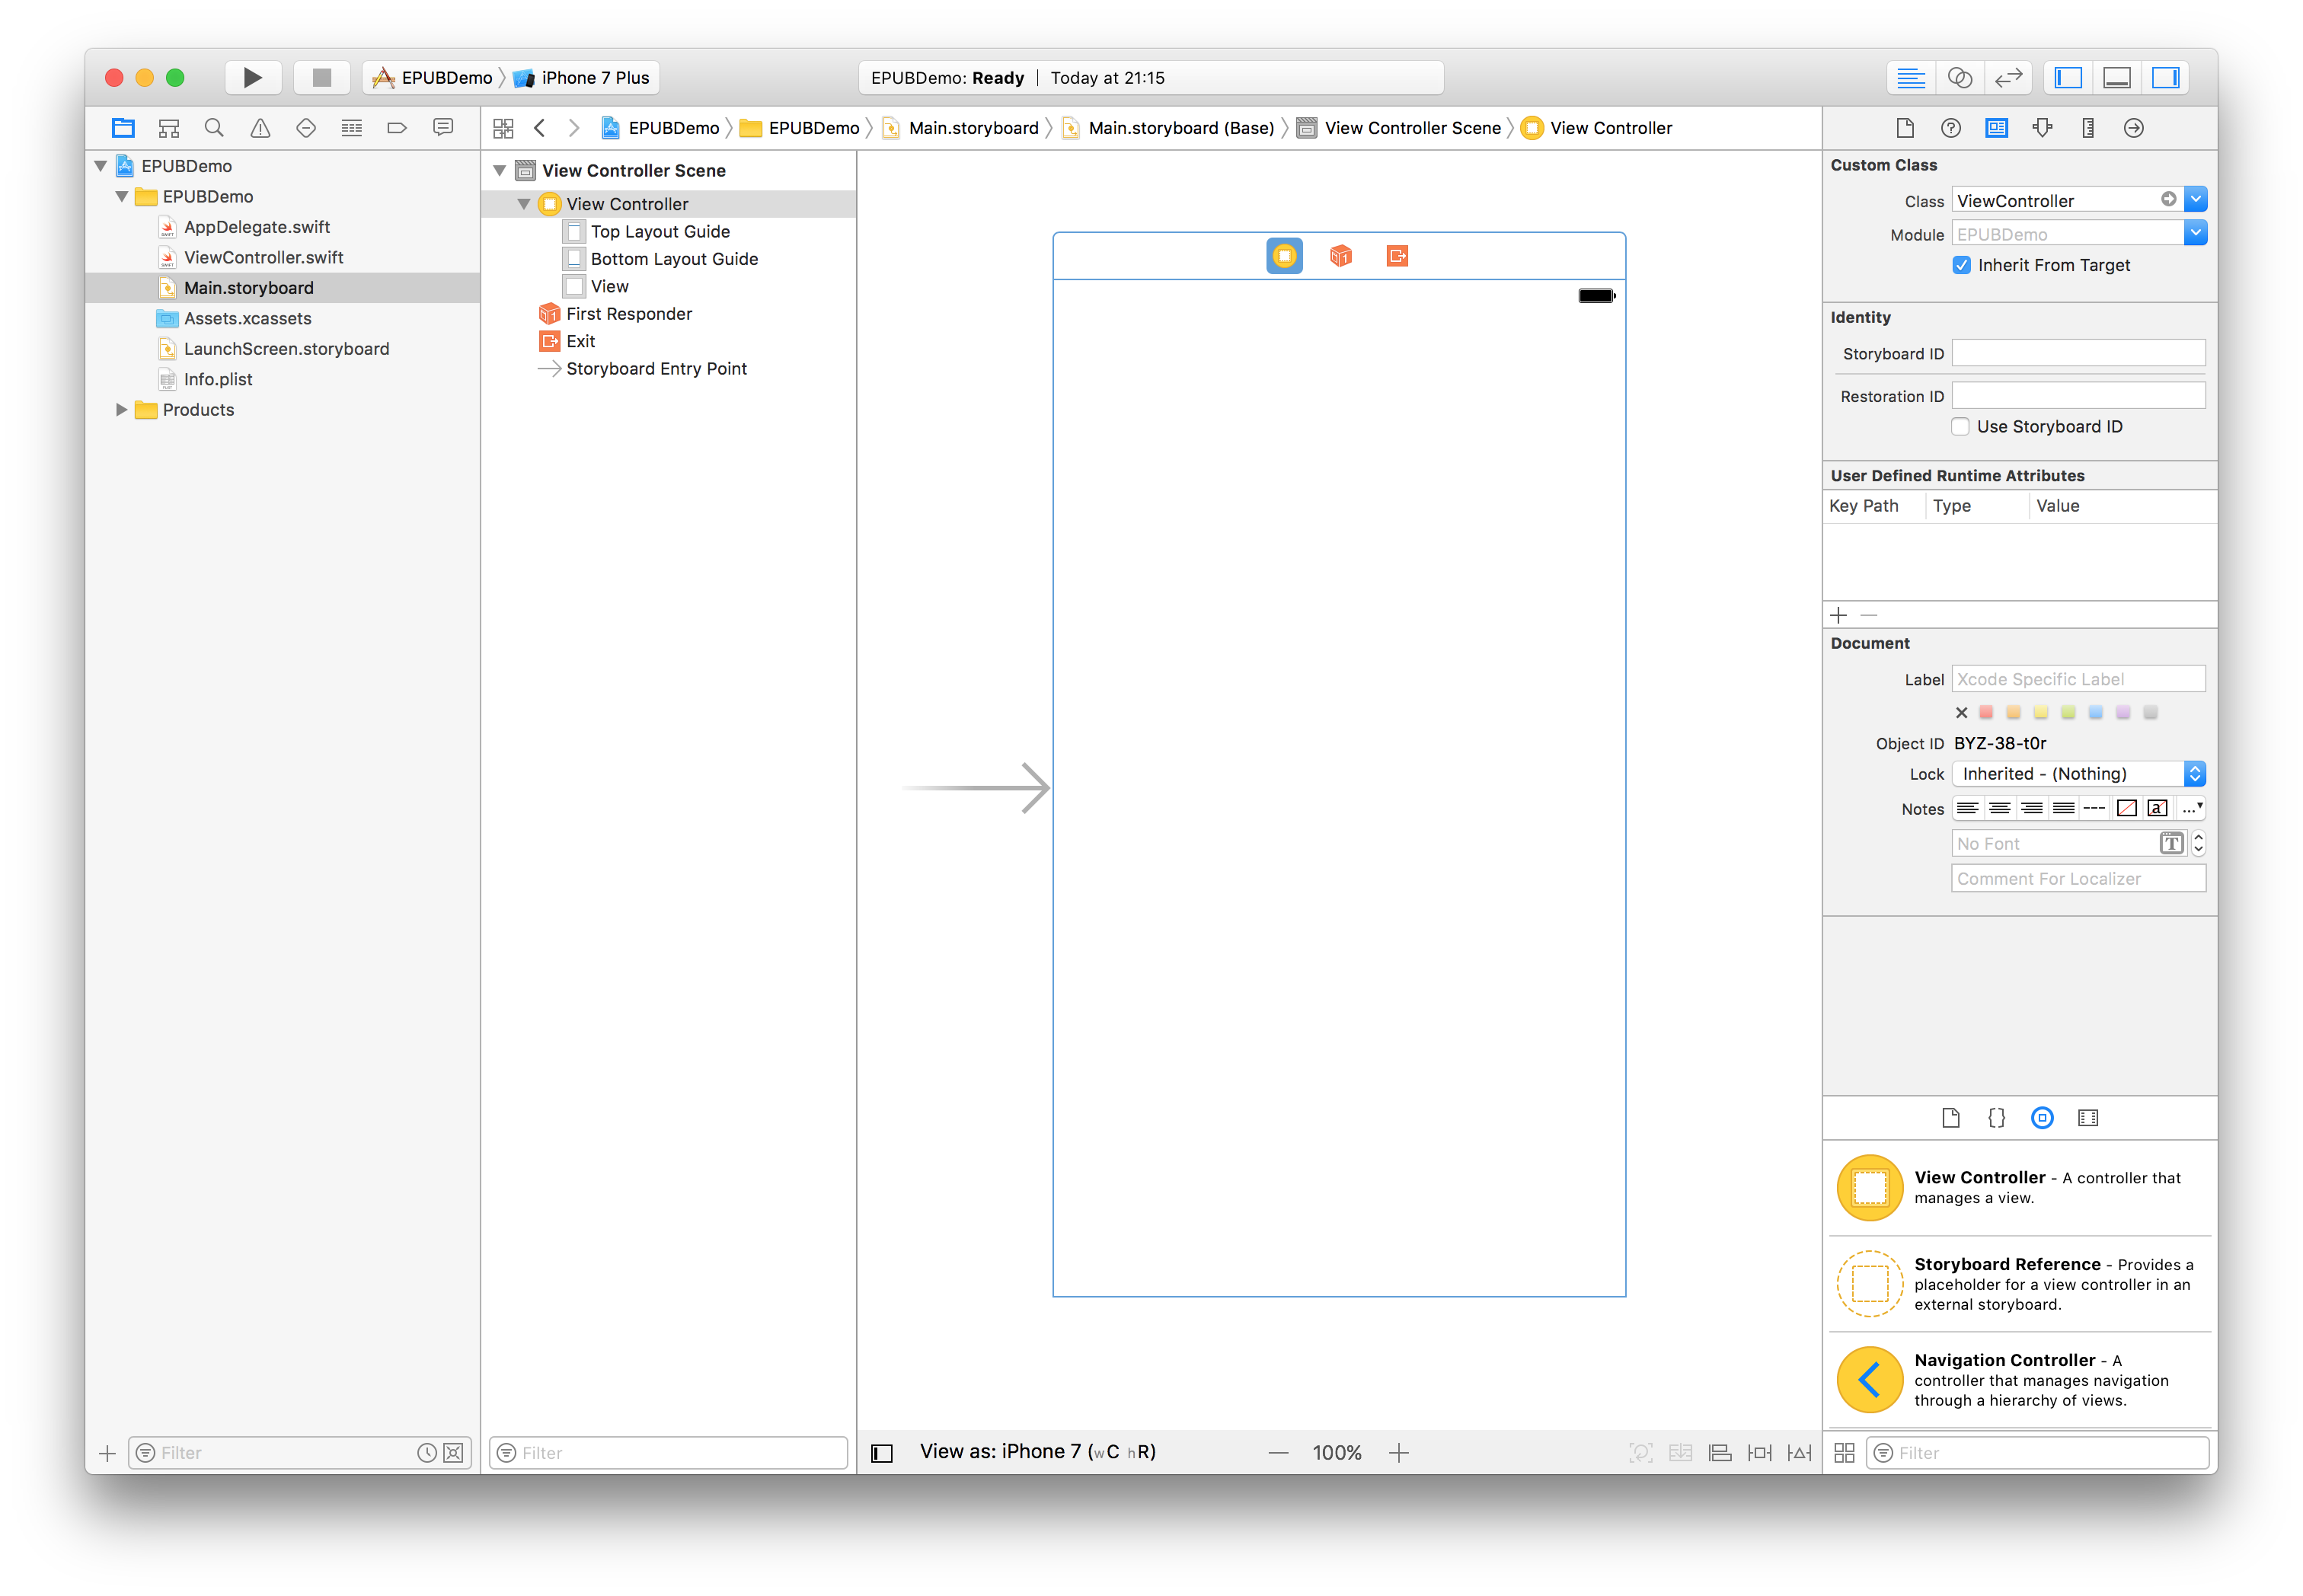
\includegraphics[width=120mm]{images/chapter-5-image-1-storyboard.png}
  \caption{Plik \textit{Main.storyboard} wyświetlony w Xcode.}
  \label{chapter-5-image-1-storyboard}
\end{figure}

Aplikacja będzie zbudowana przy pomocy \textit{storyboardów} widocznych na rysunku \ref{chapter-5-image-1-storyboard}, dzięki którym w prosty sposób można zaprojektować interfejs użytkownika przy pomocy gotowych komponentów, które można modyfikować według upodobań. Zanim jednak wytłumaczę jak zaprojektować widok w \textit{storyboardach}, należy poruszyć ważną sprawę, którą należy dobrze przemyśleć przed podejściem do programowania i komponowania widoku. Mam na myśli schemat \textit{Model-Widok-Kontroler}, który każdy widok aplikacji posiada przynajmniej jeden. Tworzenie widoku należy rozpocząć od ustalenia co będzie naszym modelem, a co będzie widokiem. Należy pamiętać, aby model i widok były rozdzielone i nigdy się ze sobą nie komunikowały, ponieważ to kontroler decyduje w jaki sposób wyświetlić dane modelu na widoku. Między modelem, a widokiem istnieje niewidoczna linia, która nigdy nie może zostać przekroczona. To podejście pozwala nam w efektywny sposób zaprojektować architekturę aplikacji składającą się z wielu \textit{MVC}, a to zapewni znakomitą organizację kodu.

Zatem zastanówmy się co będzie naszym \textit{MVC}. Pierwszy widok będzie przedstawiał listę książek, które znajdują się w aplikacji. W przypadku wybrania jednej z nich zostaniemy przeniesieni do widoku który dostarcza \textbf{EPUBKit}. Modelem pierwszego widoku więc będą książki zawarte w aplikacji, a książki naturalnie będą w formie instancji klasy \texttt{EPUBDocument}, którą również dostarcza \textbf{EPUBKit}. Widokiem jak już wspomniano będzie lista, a więc użyjemy komponentu \texttt{UITableView}, który pozwala na wyświetlenie komórek jedna pod drugą. \texttt{UITableView} dziedziczy z klasy \texttt{UIScrollView} co zapewnia naszej tabeli możliwość przewijania. Chcielibyśmy aby każda komórka w tabeli reprezentowała jedną z książek zawartych w aplikacji. Dobrze by było aby komórka ta poza tytułem książki wyświetlała również autora oraz miniaturkę okładki. W tym celu rozszerzymy klasę \texttt{UITableViewCell} w celu stworzenia własnej klasy która będzie spełniała założone wymagania, reprezentując prototypową komórkę zaprojektowaną przy użyciu \textit{Xibów}. Kontrolerem będzie własna klasa \texttt{ViewController} rozszerzająca klasę \texttt{UIViewController} (\textit{View Controllerem}, którą określa się kontener agregujący widoki, tak jak przedstawiono na rysunku \ref{chapter-5-image-2-viewcontroller-relationship}). Deklaruje między innymi metody wywoływane w każdym z momentów cyklu życia \textit{View Controllerem} reprezentującego jedno \textit{okno} widoczne w \textit{storyboardach}. Nie należy nazywać \textit{View Controller’a} oknem. Użyłem tego słowa, aby określić wizualną reprezentację \textit{View Controller’a}. \textit{Okno} reprezentowane przez klasę \texttt{UIWindow}, w nomenklaturze programowania na iOS jest instancją w której znajdują się wszystkie \textit{View Controller’y}.

\begin{figure}[ht!]
  \centering
  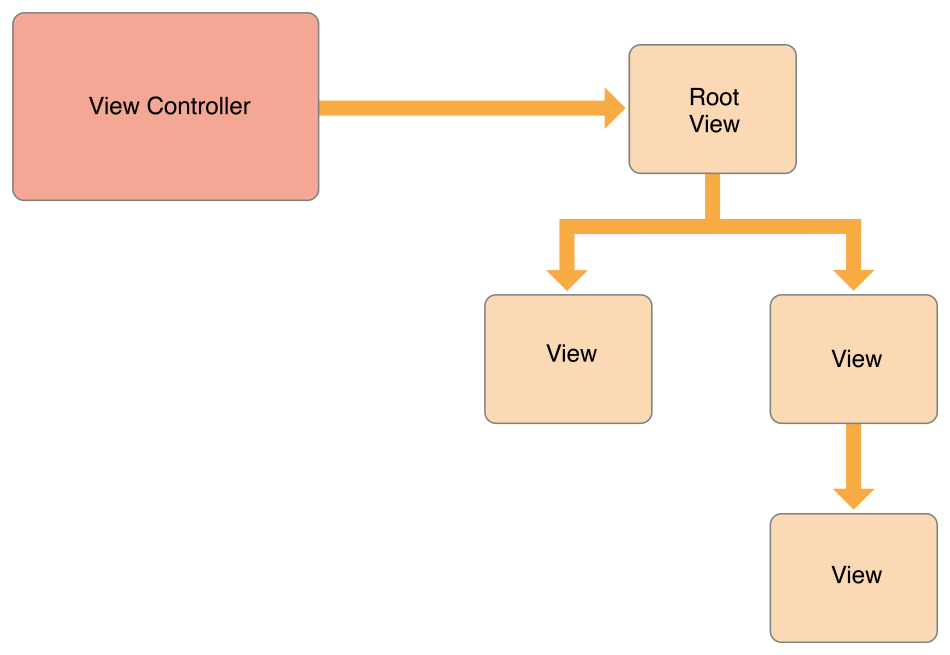
\includegraphics[width=120mm]{images/chapter-5-image-2-viewcontroller-relationship.png}
  \caption{Związek \textit{View Controllera} z jego widokami\cite{viewControllerProgrammingGuideforiOS}}
  \label{chapter-5-image-2-viewcontroller-relationship}
\end{figure}

Skoro \textit{MVC} widoku zostało ustalone, można rozpocząć jego tworzenie, a ponieważ wykorzystanie biblioteki zostanie przedstawione w kolejnym podrozdziale, zacznę od kompozycji widoku. Na głównym widoku \textit{View Controllera} upuszczam element interfejsu \texttt{UITableView}, a następnie ustawiam go względem widoku nadrzędnego, przyczepiam go do jego granic z odległością \textbf{0 pikseli}, co oznacza, że \texttt{UITableView} będzie rozszerzało się wraz z nim, przez co zawsze będzie rozciągnięte na całym ekranie i zachowa swoje proporcje niezależnie od rozdzielczości ekranu urządzenia oraz jego orientacji. Następnie włączam \textit{Assistant editor} w Xcode, dzięki czemu obok pliku \textit{Main.storyboard} widoczny jest plik \textit{ViewController.swift} tak jak jest to zaprezentowane na rysunku \ref{chapter-5-image-3-xcode-assistant}. Klasa \texttt{ViewController} reprezentuje \textit{View Controller} widoczny w \textit{storyboardach} (tak jest ustawione w jego właściwościach), dlatego Xcode pozwoli na stworzenie referencji między świeżo umieszczonym \texttt{UITableView}, a klasą \texttt{ViewController}. W tym celu należy przytrzymać klawisz \textit{crtl} na klawiaturze i przeciągnąć myszką chwytając element w \textit{storyboardach} i upuszczając go w klasie odpowiadającej danemu \textit{View Controllerowi}. Zostanie wyświetlone okienko dialogowe na którym trzeba ustawić szczegóły referencji która ma zostać stworzona. Finalnie w klasie pojawi się zmienna oznaczona atrybutem \texttt{@IBOutlet} odnosząca się do wcześniej stworzonego elementu w \textit{storyboardach}.

\begin{figure}[ht!]
  \centering
  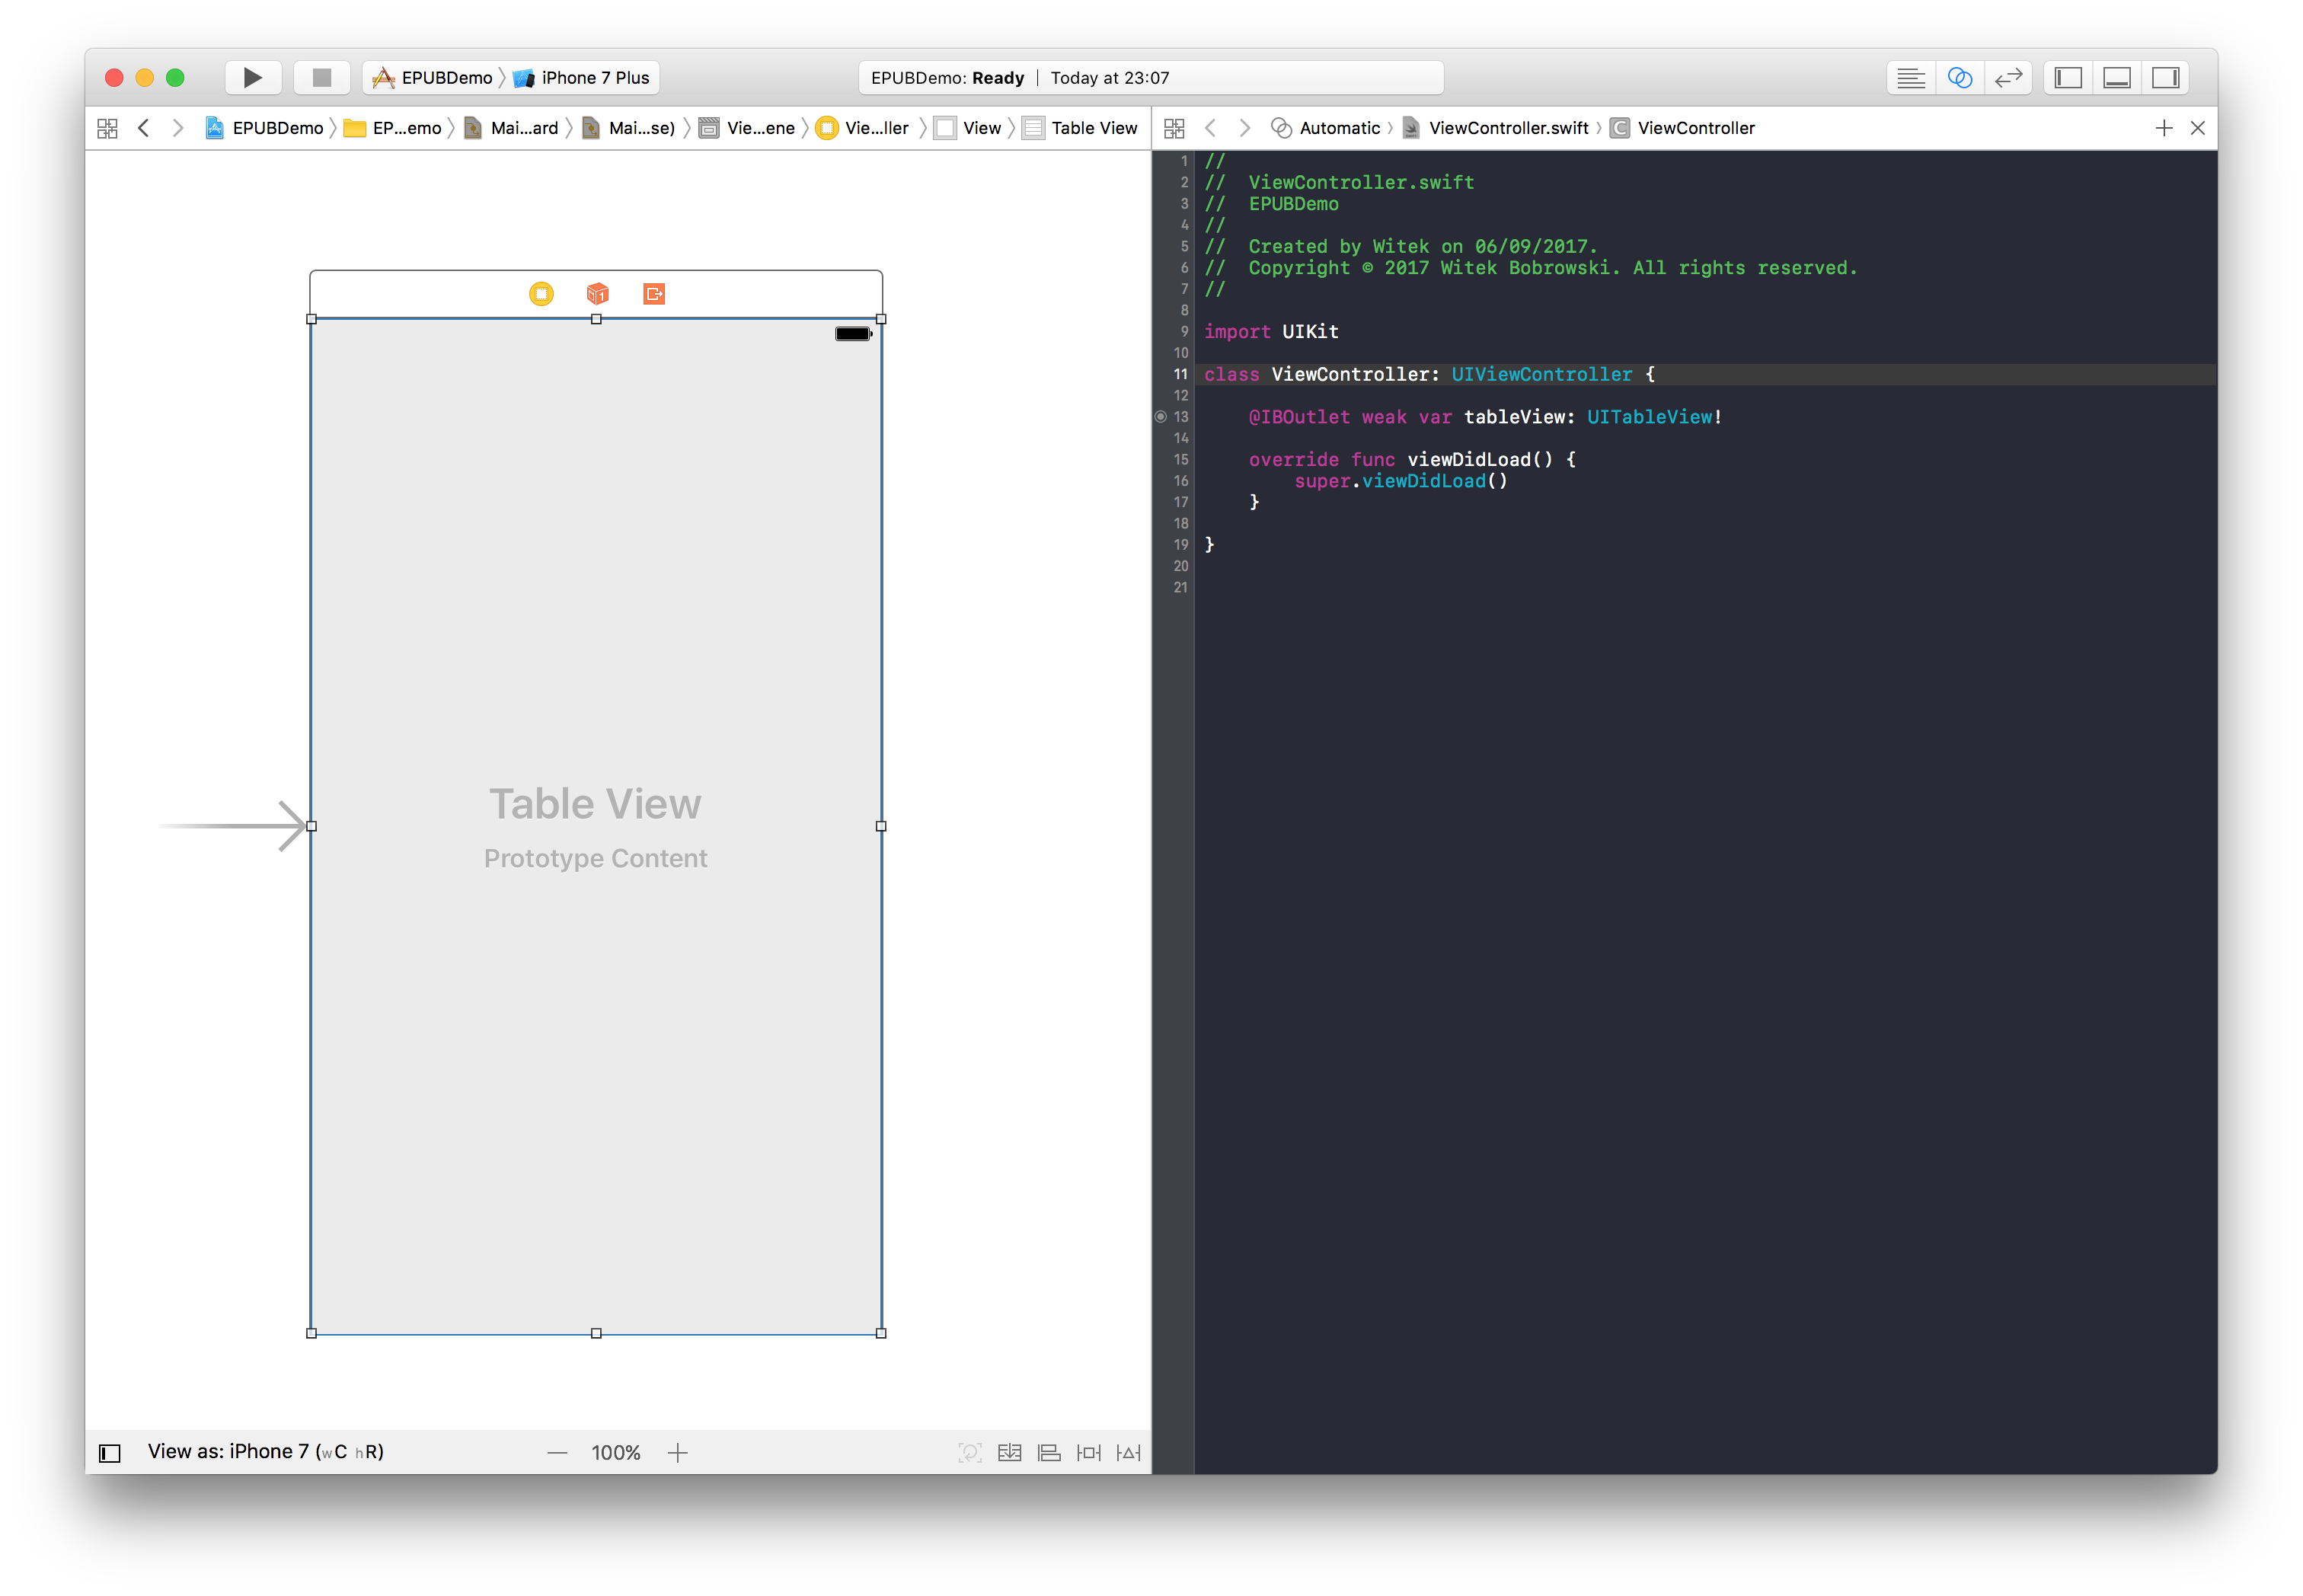
\includegraphics[width=120mm]{images/chapter-5-image-3-xcode-assistant.png}
  \caption{Dzięki asystującemu edytorowi, Xcode pozwala na podgląd dwóch plików jeden obok drugiego}
  \label{chapter-5-image-3-xcode-assistant}
\end{figure}

Następnie można przejść do zaprojektowania komórki, której instancję będą wyświetlane w tabeli. W tym celu zostanie stworzona nowa klasa \texttt{BookTableViewCell} dziedzicząca po \texttt{UITableViewCell}, oraz plik \textit{BookTableViewCell.xib} w którym zaprojektuję widok komórki sposobem znanym ze \textit{storyboardów}. Widok ten będzie posiadał instancję \texttt{UIImageView} reprezentującą widok przeznaczony do wyświetlania obrazów oraz dwie instancje \texttt{UILabel}, elementu przedstawiającego etykietę. Jak można zaobserwować na rysunku \ref{chapter-5-image-4-book-cell}, widok w pliku \textit{Xib} ma określoną klasę reprezentującą siebie, co jest absolutnie wymagane jeżeli zamierzamy użyć tego widoku w aplikacji.

\begin{figure}[ht!]
  \centering
  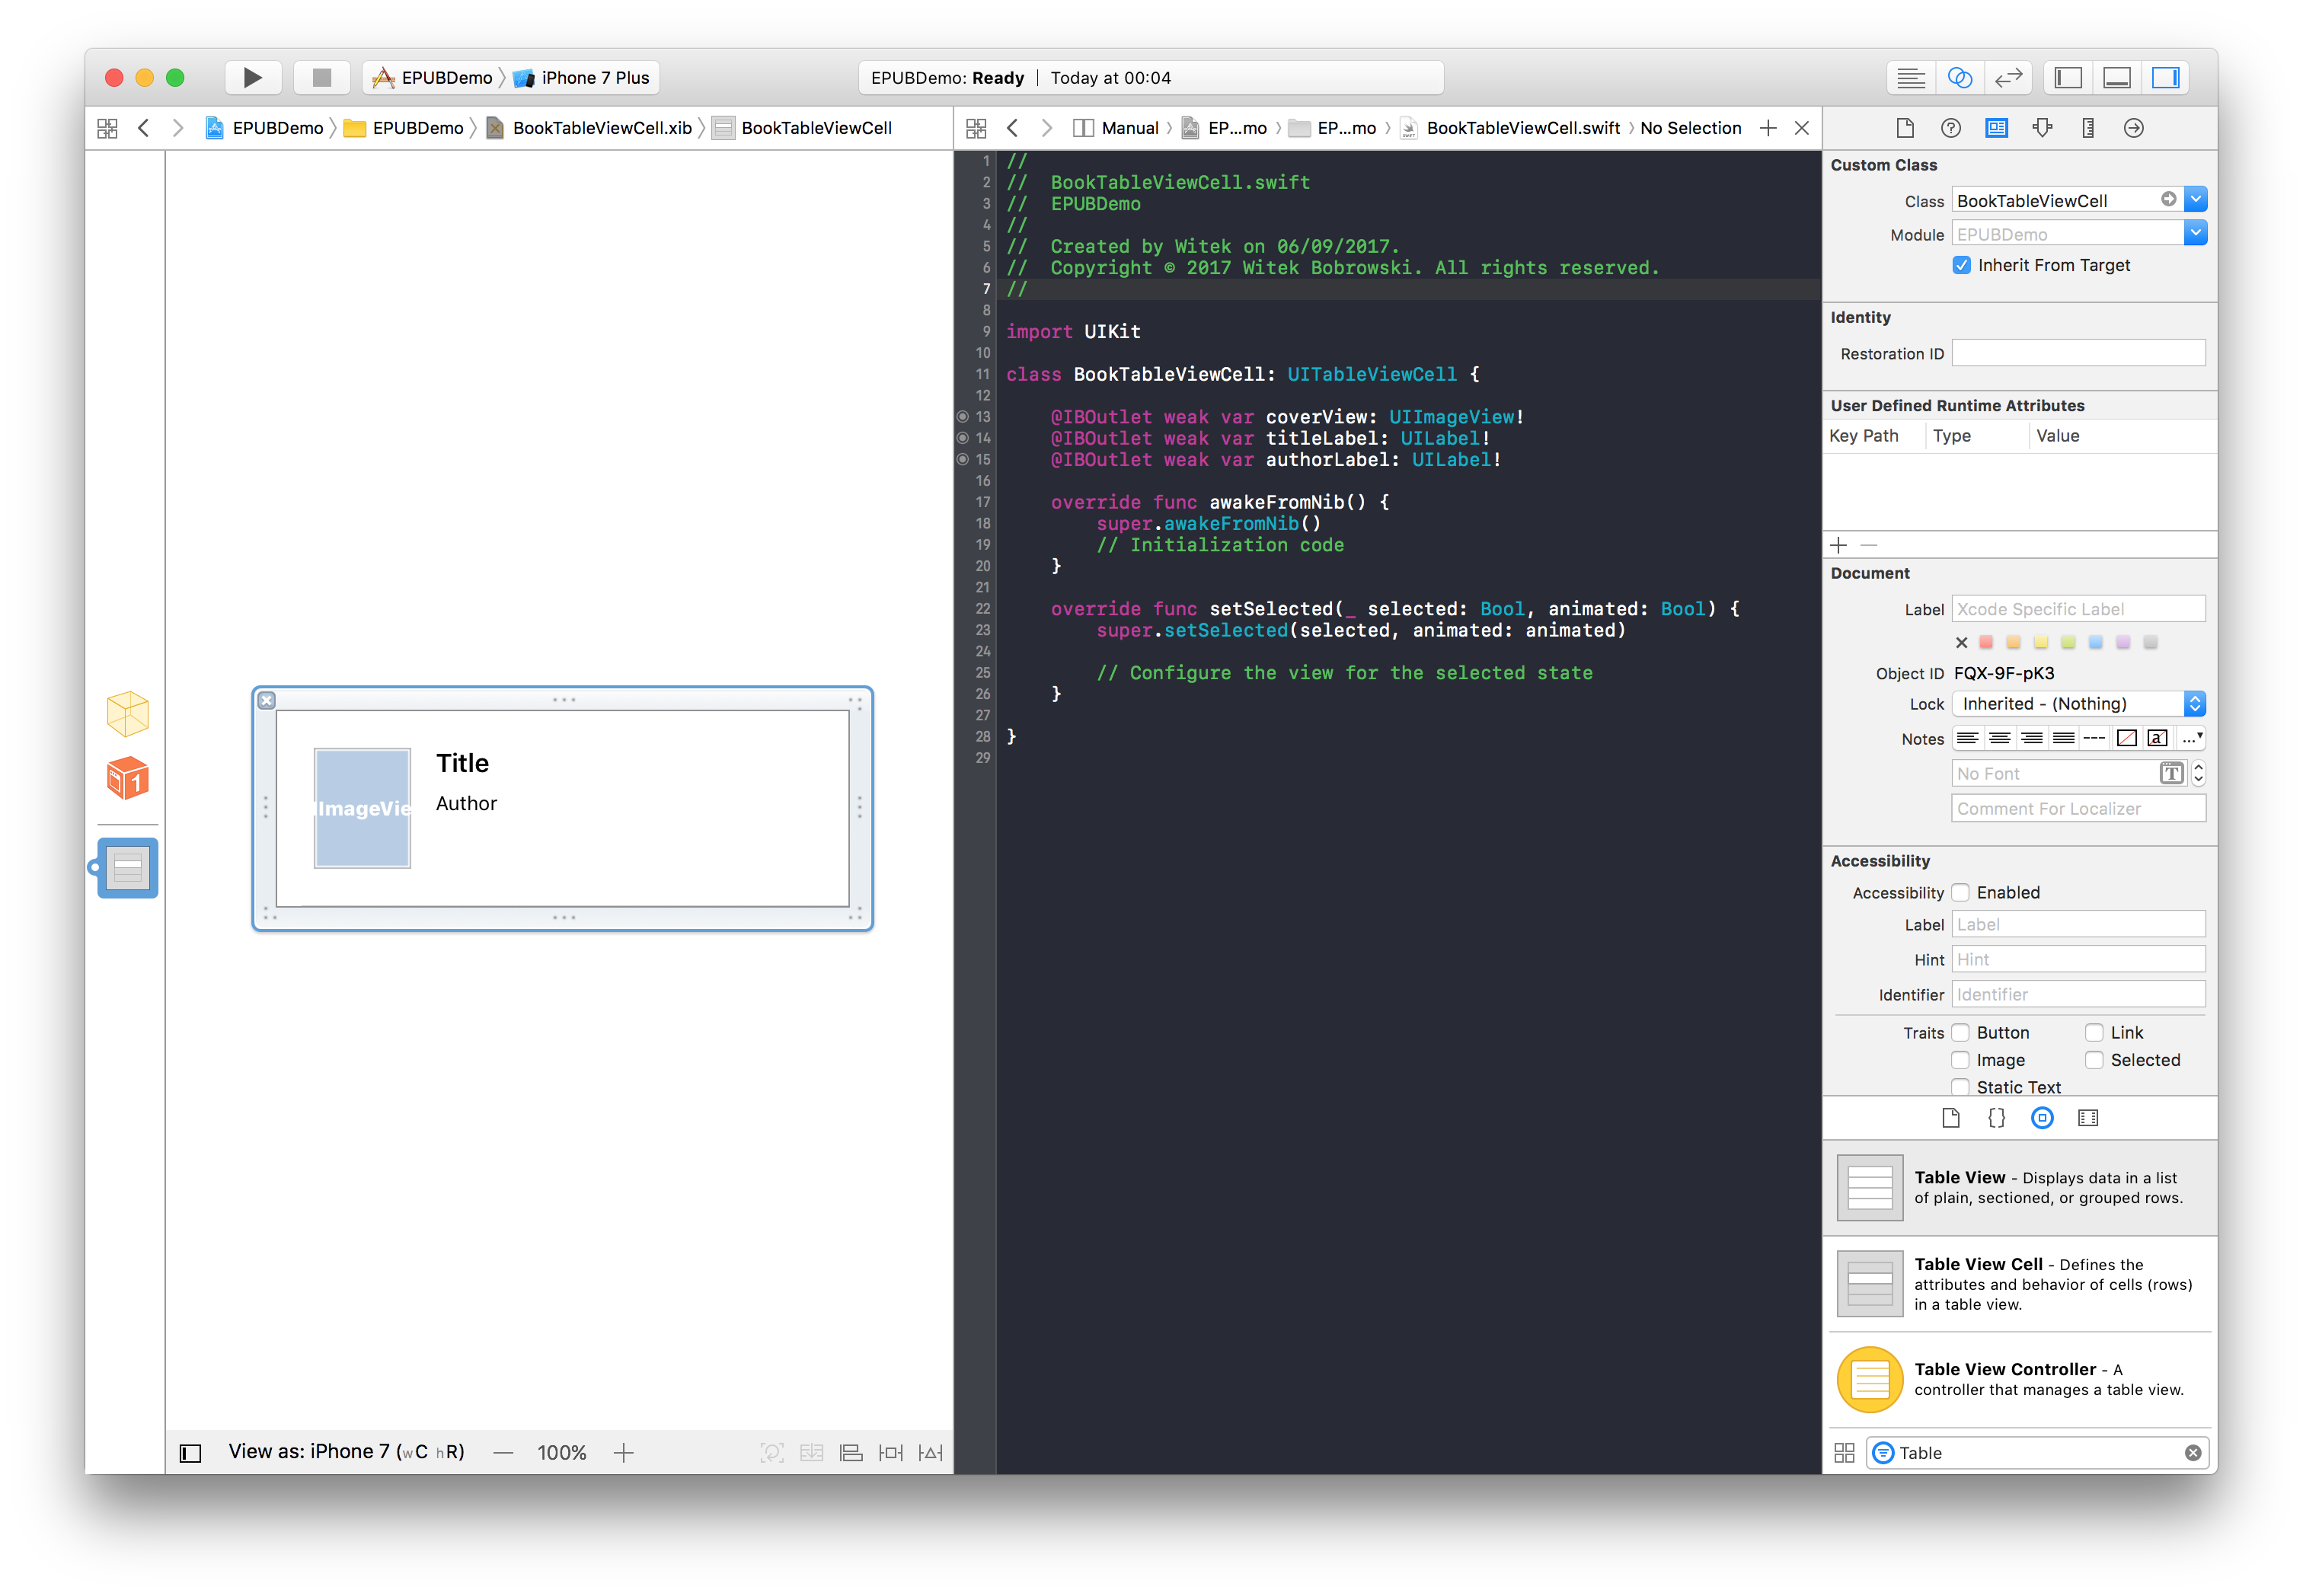
\includegraphics[width=120mm]{images/chapter-5-image-4-book-cell.png}
  \caption{Pliki \textit{Xib} pozwalają na zaprojektowanie niezależnego widoku}
  \label{chapter-5-image-4-book-cell}
\end{figure}

\section{Wykorzystanie biblioteki w aplikacji}

Aby zaimplementować logikę aplikacji, należałoby w tym miejscu dołączyć bibliotekę \textbf{EPUBKit} do przestrzeni roboczej aplikacji. W tym celu należy zainstalować menadżera paczek \textit{CocoaPods} i zainicjalizować \textit{pods’y} w folderze zawierającym projekt \textbf{EPUBDemo} przy pomocy komendy \textit{pod init}. Ta instrukcja stworzy plik \textit{Podfile}, w którym będziemy trzymać referencje zależności aplikacji. Pierwszą z nich będzie naturalnie \textbf{EPUBKit}, więc plik \textit{Podfile} powinien wyglądać tak jak na wykazie \ref{Podfile}. Nastepnie należy po raz kolejny przejść do terminalu i uruchomić komendę \textit{pod install}, która zainstaluje wszystkie wymienione w \textit{Podfile} zależności i stworzy dedykowaną dla projektu przestrzeń roboczą. W tym momencie należy wyłączyć Xcode jeżeli uruchomiony jest plik projektu, i otworzyć nową przestrzeń roboczą. \textbf{EPUBKit} został zainstalowany, i jest gotowy do użytku, a więc można go zaimportować instrukcją \texttt{import EPUBKit} w dowolnym pliku źródłowym swift.

\begin{lstlisting}[caption={Struktura modelu EPUBKit}, language=bash,label=Podfile]
source 'https://github.com/CocoaPods/Specs.git'
platform :ios, '10.3'
use_frameworks!
target 'EPUBDemo' do
  pod 'EPUBKit', :git => 'https://github.com/witekbobrowski/EPUBKit.git'
end
\end{lstlisting}

\subsection{BookTableViewCell}

Komórka tabeli wyświetlającej książki, jest relatywnie prostym widokiem. Klasa nie wymaga skomplikowanej konfiguracji, a poza referencjami widoków znajduje się tutaj wyłącznie jedna własność, która odnosi się do konkretnej instancji \texttt{EPUBDocument}. Jak przedstawiono na wykazie \ref{BookTableViewCell}, w momencie nadpisania własności \texttt{epubDocument}, wywołana zostanie metoda konfiguracji, i wypełni ona widok danymi.

\begin{lstlisting}[caption={Deklaracja klasy \texttt{UITableViewCell}}, language=swift, label=BookTableViewCell]
class BookTableViewCell: UITableViewCell {
    @IBOutlet weak var coverView: UIImageView!
    @IBOutlet weak var titleLabel: UILabel!
    @IBOutlet weak var authorLabel: UILabel!
    public  var epubDocument: EPUBDocument? {
        didSet {
            configure()
        }
    }
}
//MARK: Configuration
extension BookTableViewCell {
    fileprivate func configure() {
        titleLabel.text = epubDocument?.title
        authorLabel.text = epubDocument?.author
        coverView.contentMode = UIViewContentMode.scaleAspectFit
        if let cover = try? UIImage(data: Data(contentsOf: epubDocument?.cover ?? URL(fileURLWithPath: "") )) {
            coverView.image = cover
        }
    }
}
\end{lstlisting}

\subsection{ViewController}

Główny widok aplikacji, czyli lista książek została zadeklarowana w sposób widoczny na wykazie \ref{ViewController-1}. Definiuje on zmienną \texttt{availableBooks}, która jest tablicą przechowującą nazwy plików .epub dostępnych w aplikacji. W tym rozdziale nie będę omawiał ani konfiguracji widoku, ani organizacji modelu danych dla tabeli.

\begin{lstlisting}[caption={Deklaracja klasy \texttt{UIViewController}}, language=swift, label=ViewController-1]
class ViewController: UIViewController {
    @IBOutlet fileprivate weak var tableView: UITableView!
    fileprivate var availableBooks: [String] = []
    fileprivate var model: [EPUBDocument] = [] {
        didSet {
            tableView.reloadData()
        }
    }
    override func viewDidLoad() {
        super.viewDidLoad()
        configure()
        rebuildModel()
    }
}
\end{lstlisting}

To co natomiast chciałbym poruszyć, to sposób inicjalizowania widoku z biblioteki \textbf{EPUBKit}. Otóż w celu przeniesienia się do widoku dokumentu, w pierwszej kolejności użytkownik musi wybrać odpowiednią pozycję w tabeli, co wywoła metodę delegata, której implementacja została przedstawiona na wykazie \ref{ViewController-2}.

\begin{lstlisting}[caption={Deklaracja metody delegata \texttt{UITableView}}, language=swift, label=ViewController-2]
func tableView(_ tableView: UITableView, didSelectRowAt indexPath: IndexPath) {
    let bundle = Bundle(identifier: "org.cocoapods.EPUBKit")
    if bundle != nil {
        let ekViewController = UIStoryboard(name: "Main", bundle: bundle).instantiateViewController(withIdentifier: "EKViewController") as! EKViewController
        ekViewController.epubDocument = model[indexPath.row]
        navigationController?.pushViewController(ekViewController, animated: true)
    }
}
\end{lstlisting}

W momencie wybrania któregoś z rzędów w tabeli, metoda delegata zainincjalizuje kontroler \texttt{EKViewController} przy pomocy instancji klasy \texttt{Bundle}, dzięki której otrzymujemy dostęp do plików znajdujących się w bibliotece. Następnie przypisujemy do własności stałej \texttt{ekViewController} dokument \texttt{EPUBDocument}, aby na końcu nałożyć nowy kontroler na kontroler nawigacji, co skutkuje pojawieniem się widoku już znanego i omówionego w poprzednim rozdziale. Jedyne co pozostało to przerzucić do projektu aplikacji pliki EPUB, i uwzględnić ich nazwę bez rozszerzenia, w tablicy \texttt{availableBooks} oraz uruchomić aplikację.

To jest cała logika, którą wykonać musi aplikacja. Zainicjalizować instancję \texttt{EPUBDocument} oraz stworzyć widok z paczki biblioteki. Pierwotne założenie zostało spełnione, to znaczy udało się stworzyć bibliotekę, dzięki której można w bardzo prostu sposób stworzyć obiekt dokumentu EPUB, a następnie go wyświetlić.
